\section{Traffic Simulation Software}

The basis for the implementation will be set by a traffic simulation software. The requirements for this software were defined in \ref{trafficSimulationRequirements}. Based on an internet research the three traffic simulators CityTrafficSimulator, MATSim and CORSIM were preselected and will now be compared with the ten requirements.

CityTrafficSimulator is a traffic simulation software for small- to medium-sized traffic networks. It implements the intelligent driver model.\footcite{citation needed (traffic-simulation.de)} The simulation does not support pedestrian traffic, but this could theoretically be implemented by the user, because CityTrafficSimulator is open source.

The simulation results are shown visually and can also be extracted with different metrics. It would also be easy to extend the visuals of the simulation and extract arbitrary data from the network, because as stated earlier the project is open source.

CityTrafficSimulator has traffic lights built in, but it has no application programming interface for dynamic traffic light controllers, but as with the extraction of arbitrary data this could be implemented.

A unique aspect of CityTrafficSimulator to the other two traffic simulations is its Signal Light Editor, which allows the user to model signal groups and signal times visually. MATSim for example has configuration files for this, which are harder to set up for quick testing.

The second option for the traffic simulation is MATSim, an open source traffic simulation written in Java. It has built in support for car traffic simulation, but not for pedestrian traffic. However it is possible to extend MATSim with different locomotion types. There is for example a project that simulated airplane traffic over europe with MATSim.

MATSim on its own does not have a graphical display. It only puts out log files of what happened in the process of the simulation. However there is an extension that displays in real time what is happening in the simulation. It is called OTFVis. This extension as it is open source too can be expanded by the user.

\begin{figure}[!ht]
  \centering
  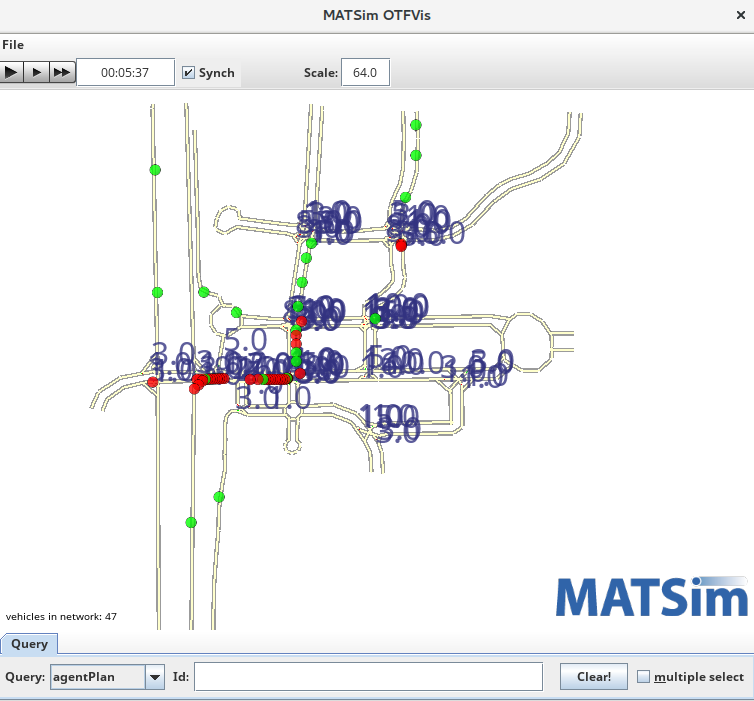
\includegraphics[width=12cm]{figures/otfvis}
  \caption[Screenshot of OTFVis]{Screenshot of OTFVis \protect\footnotemark}
  \label{otfvis}
\end{figure}

\footnotetext{screenshot}

Figure \ref{otfvis} shows the extension OTFVis for MATSim with debugging output patched in. It uses OpenGL to render to the screen and is relatively easy to extend with text output.

MATSim has different events and data structures that allow to interface with the simulation and read and write data from and to the simulation. The open source nature of MATSim also allows to expose all information wanted by compiling a custom version of MATSim.

MATSim has no built in traffic sensors or traffic lights, but like for the visual output, for traffic lights there is an extension that also allows for the dynamic control of the traffic lights.

CORSIM is the only of the three traffic simulations, discussed here that is not open source. This limits the possibilities when using CORSIM. CORSIM is also able to simulate vehicle, but no pedestrian traffic. It has a real time visual representation of the traffic simulation.

CORSIM has a built in traffic controller that uses static plans, but it is possible to use an own dynamic traffic light controller.

For custom extensions CORSIM has Run-Time Extensions (RTE) with different CORSIM Call Points which allow the extension to hook into CORSIM during execution. Examples for Call Points would be ``Initialize'', which is called at the start of the simulation, or ``PreNetsimSignal'', called each time just before the signals in the road network are updated.\footcite{
%http://sites.poli.usp.br/ptr/lemt/CORSIM/RTE%20Developers%20Guide.pdf
}

Run-Time Extensions can access data trough the CORSIM application programming interface and all the data structures used by CORSIM internally, allowing the user to extract arbitrary data.\footcite{
%http://sites.poli.usp.br/ptr/lemt/CORSIM/RTE%20Developers%20Guide.pdf
}

%http://www.cszb.net/
%https://github.com/Schulteatq/CityTrafficSimulator/tree/master/CityTrafficSimulator

\begin{table}[!ht]
  	\centering
  	\begin{tabular}{l|l|l|l}
		 & CityTrafficSimulator & MATSim & CORSIM \\[10pt]
		 \hline\hline
		Requirement & & & \\[10pt]
		\hline
		R1 & yes & yes & yes \\[10pt]
		R2 & possible & possible & no \\[10pt]
		R3 & yes & possible & yes \\[10pt]
		R4 & possible & possible & no \\[10pt]
		R5 & possible & yes & yes \\[10pt]
		R6 & no & no & no \\[10pt]
		R7 & yes & possible & yes \\[10pt]
		R8 & possible & possible & possible \\[10pt]
		R9 & yes & possible & yes \\[10pt]
		R10 & no & no & no \\[10pt]
		Other & & & \\[10pt]
		\hline
		Open Source & yes & yes & no \\[10pt]
		Prog. Language & C\# & Java & C++, FORTRAN, ... \\[10pt]
	\end{tabular}
  	\caption{Traffic Simulation Software Requirement Fulfillment}
  	\label{simulationRequirementsComparison}
\end{table}

Table \ref{simulationRequirementsComparison} summarizes the result of the traffic simulator comparison. The value ``possible'' means that it is not included in the main program, but can be done through some external program or extension.

MATSim was chosen as the simulation for the traffic light control system. As can be seen in table \ref{simulationRequirementsComparison}, all three traffic simulations have almost the same feature set regarding the requirements, but in comparison to CORSIM, MATSim was chosen, because it is open source and with a project that might have to expand on the simulation it uses, open source fits really well to the traffic signal control system. In comparison to CityTrafficSimulator, MATSim with the extensions OTFVis and Signals, both fulfilled the same requirements, but the community surrounding MATSim, the other extensions and the whole feature set is more complete.

\subsection*{Dependency Injection}

The MATSim software is currently in the migration phase of switching from manual (compile-time) dependency to runtime dependency injection using the Guice Framework developed by Google. Extensions can be developed as a separate dependency injection module for Guice providing additional class bindings. This is what has been done for this project as well. The project is linked against the required matsim modules and provides a new module that installs all interfaces and implementations into the injector. The module takes parameters for default bindings which can be supplied manually, if the project is used as a library, or automatically from command line parameters.

Due to problems with the dependency injection module of OTFVis, the visualization component, probably caused by an incomplete migration, it was necessary to completely recreate parts of the component's initialization code in order to be able to start the visualization.

\section{Scenario generation}
\label{scenario_generation}

An important part of the implementation of this project is to generate a test scenario with a street network with signals and also actual drivers, which in the context of simulations are often called agents, that move through the street network.

\subsection*{The Network}

MATSim offers multiple ways to create a simulation network. Networks are defined as XML files, that define nodes and links. Nodes are just points at a specific location in the simulation space. Links are directed connections between two nodes. In addition to the origin node and the destination node, these links have additional attributes attached to them. A link can have multiple lanes, a certain speed limit, the capacity in vehicles per hour and a length. Defining the length of links might seems odd at first, but it is a useful way to abstract away irrelevant details of the a street network. For example when a street network is imported from an external source, the network might be a close reconstruction of the real world streets with all the curves and corners. However this simulation is only interested in the intersections of the network, so nodes where two or more links come to together or split apart. All other links and node can be merged together, as seen in \autoref{complicated_vs_simple}. In order to still preserve the driving distance of the connection, the lengths of the individual links are added up and assigned to the new link.

\begin{figure}[ht!]
	\centering
	\includegraphics[width=12cm]{figures/complicated_vs_simple}
	\caption{Detailed street network (left side) compared to an structurally equivalent simple network}
	\label{complicated_vs_simple}
\end{figure}

There are a few options to create networks.

\paragraph{Manually} This is the simplest approach, especially because the XML format is quite simple with just nodes and links. However writing a reasonably complicated street network from hand becomes very cumbersome very quickly and is also very error prone while making changes to the network.

\paragraph{Use a graphical editor} There are two graphical editors available to create and edit MATSim networks, both developed as part of the project. The first option is the ''NetworkEditor`` module for MATSim which is a simple Swing application that can be used to create new networks from scratch and edit existing ones. This tool is very unstable and the only assistance is a rudimentary snapping feature, that connects the new link to an existing node. Viewing and editing node and link properties is also possible. The second option is a plug-in for jOSM, a Java-based Open Street Maps editor. This editor allows to work fast and effective, but the version of the plug-in that was tested, was unable to save the created networks due to a bug in the software. Both tools do not support traffic signals.

\paragraph{Import external map data} MATSim has a converter for Open Street Maps (OSM) data as part of the core library, which produces good networks. The same converter can be used from jOSM to export the OSM data as a MATSim network, which works exactly the same, jOSM however is only useful for fairly small city sections, because the download is limited to a certain amount of elements. The main problem with the converter is the missing support for exporting traffic signals.

The main network for this simulation was built using the NetworkEditor tool, which works well enough with a enough practice. The network, seen in \autoref{otfvis}, is inspired by Mannheim's city center. It has a highway on the left connected to the main horizontal street, a set of roundabouts, five unrestricted intersection and a few T-junctions.

\subsection*{The Signals and Signal Groups}

Signals and signal groups are separate from the street network in MATSim, because signals are not a core part of the simulation as described previously. There are two data models, one data model in the simulation and one for the definition / configuration. The configuration data model is separated into three parts (with three separate XML files):

\begin{enumerate}
	\item Systems
	\item Controls
	\item Groups
\end{enumerate}

As previously mentioned, the graphical network editors available for MATSim do not support traffic signal and thus all of these configurations must be either written by hand or generated from our own code base.

\paragraph{Systems} A system is basically an intersection. It defines the the signals of one intersection and attaches them to their links. Signals are attached to link, that means in MATSim signals are attached to the input link. Vehicles can not enter any of the output links coming from the input link as long as the input link's signal is red, however they can enter the input link itself. For that reason, intersections are not actually modeled like in \autoref{unrestricted_intersection}, but actually similar to what can be seen in \autoref{actual_intersection}.

\begin{figure}[ht!]
	\centering
	\includegraphics[width=4cm]{figures/actual_intersection}
	\caption{An intersection how it's modeled in the simulation (red links have signals).}
	\label{actual_intersection}
\end{figure}

Another reason is the effect called spill-back which is preserved with this network. When vehicles from a turn lane are queuing all the way back into the normal lane before, that is what's called spill-back. \cite{matsim}

\paragraph{Controls} Systems only define the the signals of the intersection, the controls configuration assigns a signal controller class to each of the system. All systems must be assigned a controller, otherwise MATSim crashes with a \texttt{NullPointerException} (\texttt{NPE}). By default, MATSim's signals module doesn't actually support other signal controllers. Specifying something else would result in a crash once again. For this to work, the signals module got patched to apply a controller to all intersections, that was given as a command line option to the program. The signals module also expects signal controllers to work with plans with conflicts with our concept, however the simulation works without specifying plans and implementing the corresponding interfaces, so it is left that way. Otherwise a signal controller is quite simple from the API point of view: A method that receives the signal system corresponding to the controller, a method that is called once the simulation engine was initialized and finally a method that is called in every simulation step. In addition to the basic signal controller API our implementation also has the signal network controller instance which all signal controllers will report events to and receive certain events from, like signal group state changes.

\paragraph{Groups} Signal groups, as explained in \autoref{signal_group_concept}, group several signals into one control unit. This configuration defines all groups for all systems. Leaving out systems will result in a \texttt{NPE}. For large and complicated street networks this XML can grow quite large as well and become very hard to maintain and update. However with a few assumptions about the modeled street network, this file can entirely be generated without any additional information besides the network and the signal systems configuration. For the algorithm explained in the concept section, it is required to know if the lanes of two signals intersect or merge as part of the intersection. For arbitrary networks this would be a difficult problem to solve, because the progression of lanes can not generally be predicted and might require expensive graph traversals. Certain heuristics could help here, but the only guaranteed save method would be to manually specify if two signals are conflicting. As we control the street network, which was another reason not to use Open Street Maps data, we can assume two facts about the intersections in the network:

\begin{enumerate}
	\item The first link right after the signal will be used for the (geometric) intersection test. If these links to not intersect, the signals are considered intersection free.
	\item The lanes of two signals to not merge within 5 links after the signal itself, they are considered non-merging.
\end{enumerate}

Both of these assumptions apply to the intersection model used in the network as seen in \autoref{actual_intersection}.

\subsection*{The Population}

Without the population, the traffic simulation would not make sense. The street network without people driving through it would be wasted resources. In MATSim, the population of simulation scenario is defined as a set of persons. Just like in the real world, a person follows a plan. In MATSim persons have a set of different plans, but only one of these plans is selected. Such a plan consists of any number of ''act``s and ''leg``s. An act is simply a name, a location given as a reference to a link and a end time; something a person does at a given location until a certain time. Every plan starts with an act as the start point. The final act can omit the end time, because he has nothing more to do and can leave the network forever. Leg's define, how the person travels from act to act. In this simulation, only ''car`` legs are used, but different types for example for public transportation and pedestrians would be possible.

Writing this from hand is obviously not feasible. A simulation would normally use thousands of persons. For commercial research, data from statistics about the network section is used to generate a fraction of the expected traffic. Due to privacy reasons, this data is not openly available.

Another approach is to randomly generate persons passing through the network. Completely randomizing all routes (the chain of acts is basically a path through the network, as MATSim will deterministically search the shortest path between the acts) is not realistic either, because usually you have streets where more vehicles drive and streets that are less commonly used. In order to get this effect, a set POIs, Points of Interest, is defined. These POIs each consist of a type, a link id (the location) and a weight. There are four different types:

\begin{enumerate}
	\item Start: Every person will start at one of these
	\item Intermediate: These points represent places, where the person does something inside the network for a certain time
	\item No-Intermedate: This is not a point, but tells that the person will just pass through the network without explicitly stopping
	\item End: Every person will finally end his journey here
\end{enumerate}

The weight is then used to control the distribution of the POIs on the persons. Given a number of persons as a command line parameter, the software will generate the population based on the defined POIs and keep will store it for future simulation runs with the same setup.

\section{Neural Network Library}

\section{Prediction Network Implementation}

We tried the prediction network with an input for the amount of cars that want to pass, but this did introduce unnecessary complexity and the accuracy of the network went down

learning rule

artificial neural network type

\section{Traffic Tracker Implementation}

Problem with too many entities when infinitely splitting vehicles as they drive through decision points

Adding and removing vehicles from a tracked link has to be done after the simulation in the traffic tracker